\section{Apache Kafka}
\label{02:sec:title}

This section describes and explains the basics of the Apache Kafka system.
The description is based on two books: \emph{Designing Event-Driven Systems} \cite{apacheKafkaDesignDistributedSystems} and \emph{Real-Time Data and StreamProcessing at Scale} \cite{apacheKafkaDefinitiveGuide}.
Moreover, the Kafka streams subsection is based on \emph{Mastering Kafka Streams and ksqlDB Building real-time data systems} \cite{kafkaStreamsBook}.
We also used Kafka's documentation \cite{kafkaDocumentation} as the most up-to-date reference.
In these books and documentation, there can be found a more detailed explanation of Kafka itself.

Apache Kafka is an event streaming platform that offers many features like high performance, distribution, commit log service\footnote{\textbf{Commit log} 
---\ is a type of data structure that stores ordered sequences of events.}, and more.
It offers a publish/subscribe system to record streams that are similar to a message queue or enterprise messaging system.
Additionally, it stores record streams in a robust, fault-tolerant way.
Kafka also creates real-time data flows that reliably capture data transferred between systems or applications.
Kafka is widely used by many big companies like LinkedIn, Spotify, Netflix, and Uber.
\subsection{Motivation \cite{02-bachelor-thesis}}
\label{kafka:motivation}

In the past, companies had applications or systems that share large amounts of data.
Usually, these applications would provide valuable information to another application.
So, there was one source system and one target system.
But what about adding more source and target systems?
Assume an example where one has five source systems and five target systems.
Each source system needs something from each particular target system.
\begin{figure}[ht!]
    \hspace{0.01\textwidth}
    \subfigure[Source and Target systems without Kafka]{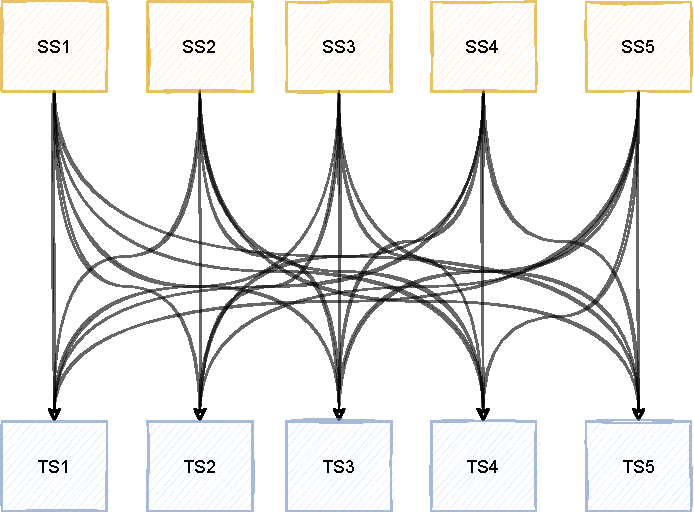
\includegraphics[scale=0.60]{obrazky-figures/02-preliminaries/02-kafka/02-kafka-without-depen.pdf}}
    \hspace{0.01\textwidth}
    \subfigure[Source and Target systems with Kafka]{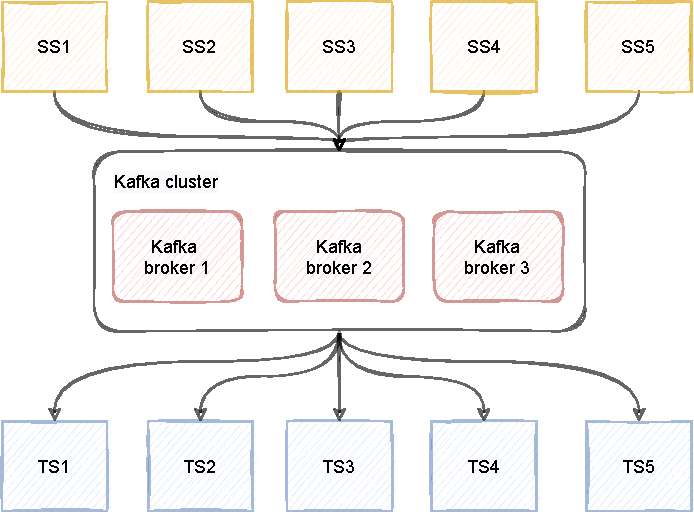
\includegraphics[scale=0.60]{obrazky-figures/02-preliminaries/02-kafka/01-kafka-with-depe.pdf}}
    \hspace{0.01\textwidth}
    \caption{How to make system more efficient with Kafka}
    \label{fig:withoutAndWithBroker}
\end{figure}

The system without Kafka depicted in Figure \ref{fig:withoutAndWithBroker}a has twenty-five links, which is not scalable (quadratic complexity).
That is onne of main reasons Kafka was invented.
Lets illustrate the same example with ten systems and Kafka in the middle serving as Middleware\footnote{\textbf{Middleware} \---\ Software, that acts as the middle man between two systems and guarantees interoperability between them.}, which is placed in the middle of these systems.
In that case, each source system only has to bind to the Kafka broker, and all data are delivered by a single link. You can see the updated system in Figure \ref{fig:withoutAndWithBroker}b.

\subsection{Fundamental concepts}

In this subsection, we describe fundamental concepts of Apache Kafka such as Producer, Consumer, Kafka broker, Kafka cluster, and so on.
The description is based on the \emph{Real-Time Data and StreamProcessing at Scale} \cite{apacheKafkaDefinitiveGuide} and Kafka documentation \cite{kafkaDocumentation}.

\begin{enumerate}
    \item \textbf{Kafka broker/cluster} \---\ it is a server application that manages messages that are sent by producers and at the same time obtained by consumers.
    In other words, it takes care of storing the data and the order of the data.
    Sometimes we can see a Kafka broker with names such as Kafka server or Kafka node.
    These names are synonymous with Kafka broker.
    Kafka broker was designed to be horizontally scalable to create a Kafka cluster (two and more Kafka brokers).
    Within a Kafka cluster, there is a single cluster controller.
    The cluster controller takes care of fundamental operations such as assigning partitions to brokers or monitoring for the failure of the Kafka brokers.
    One broker in the Kafka cluster always owns the topic partition.
    This broker is called the leader of this topic partition.
    Of course, this topic partition can be replicated into several Kafka brokers, which will result in its replication and thus data redundancy.
    On the other hand, if the leader Kafka broker fails, the one who has the replicated topic partition will take control and become the new partition leader.
    Figure \ref{02:fig:replicationOfTopicPartition} illustrates this type of scenario, where two Kafka brokers shared data between each other and partitions of the topic are replicated.

    \item \textbf{Producer} \---\ is one of the types of clients that Kafka provides.
    They produce new messages that are sent to a specific topic.
    In general, the client does not need to know to which partition it is necessary to send messages.
    It simply sends messages divided among several partitions.
    Thus, producers represent the entity that creates the data in the Kafka system.
    Kafka also provides the implementation of these clients in several languages such as Java, Go, C++, Python, and many others.
    Kafka also provides a higher level abstractions, which means that it is no longer necessary to create the producers themselves, but those entities are encapsulated in the client.
    These are, for example, Kafka Streams for stream processing or Kafka Connect API for data integration.
    
    \item \textbf{Consumer} \---\ unlike a producer, a consumer or group of consumers tries to consume messages.
    In the consumer configuration, it is necessary to specify the topic from which the consumer will read.
    However, the consumer can also read from a group of topics.
    The consumer maintains an internal offset value that represents a position from where the consumer should read the data from the topic.
    The method that consumers use to read messages is called polling\footnote{\textbf{Pooling} \---\ periodic querying to the server in that case, to the Kafka broker}.
    The consumer group behaves as an single logical unit.
    Kafka does not support reading from one specific partition more than one consumer simultaneously.
    The reason why this concept was created is based on a straightforward question - \emph{How are we able to consumes data concurrently?} Likewise, what is worth mentioning is that we \emph{can not} have more consumers than partitions because, in that type of example, some of them are inactive.
    This concept differs from other messaging solutions and describing why Kafka is so flexible in comparison with the traditional messaging based on AMQP protocol like ActiveMQ or RabbitMQ.
    
    \begin{figure}[!ht]
    \centering
    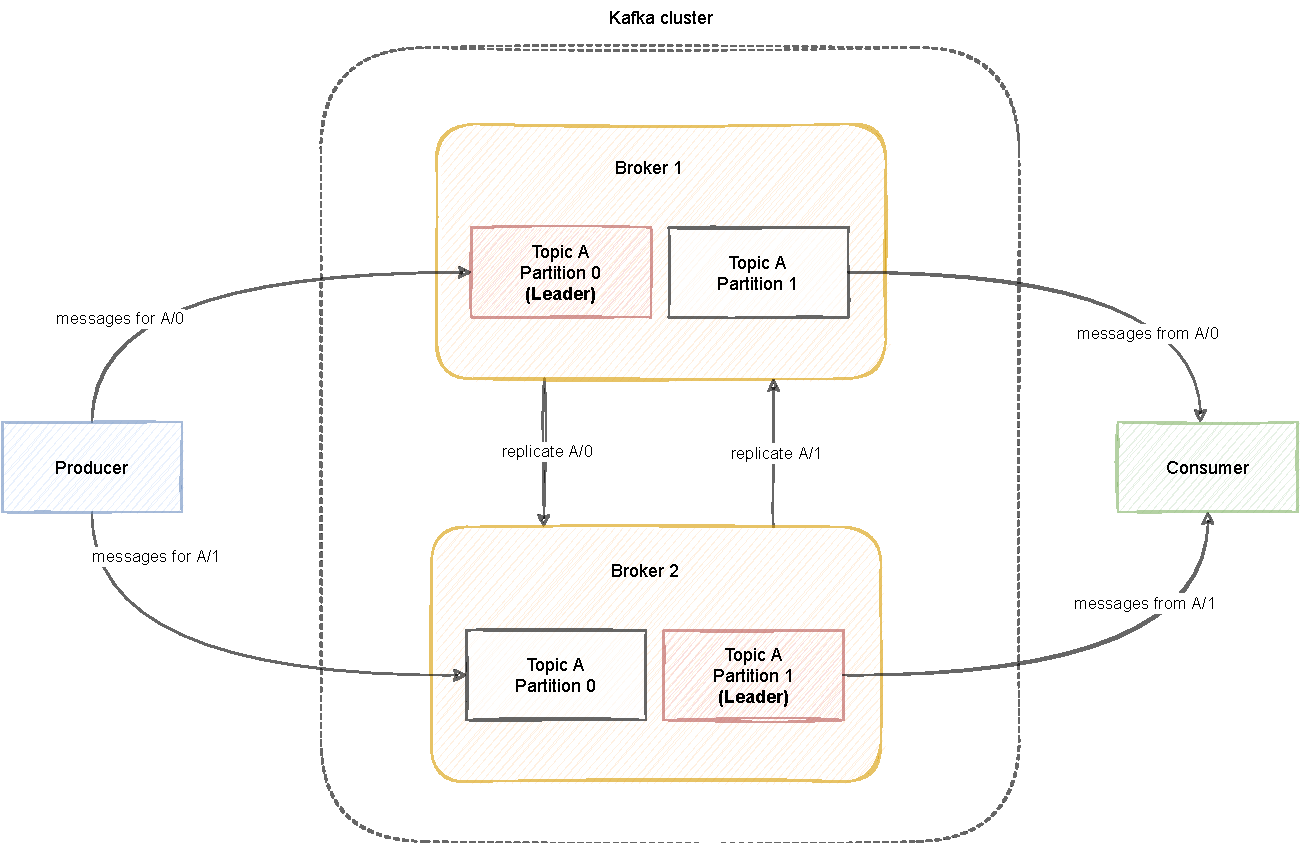
\includegraphics[scale=0.70]{obrazky-figures/02-preliminaries/02-kafka/05-replication-of-partitions.pdf}
    \caption{Kafka topic partition replication scenario in Kafka cluster inspired by \emph{Real-Time Data and StreamProcessing at Scale} \cite{apacheKafkaDefinitiveGuide}}
    \label{02:fig:replicationOfTopicPartition}
    \end{figure}

    \item \textbf{Kafka Topic} \---\ is not a simple concept and includes several parts such as the replication factor, partitions, and more.
    Kafka topic is equivalent to database table as one can see in the Figure \ref{fig:topicAndDatabaseTable}.
     \begin{figure}[!ht]
    \centering
    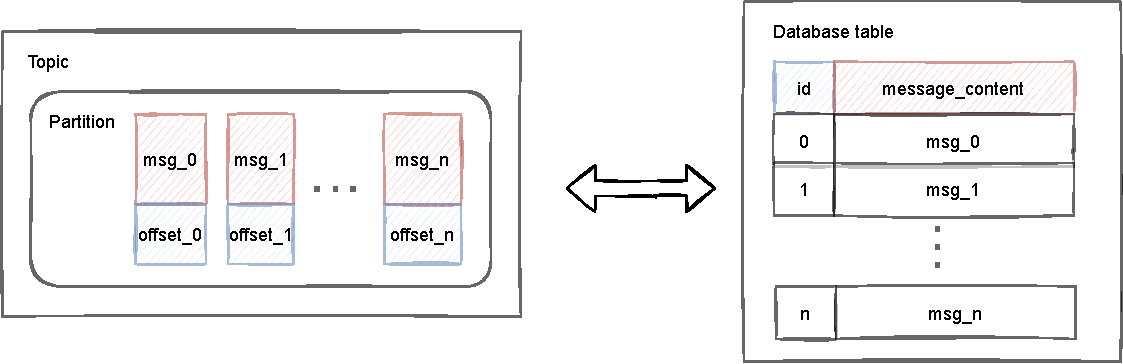
\includegraphics[scale=0.80]{obrazky-figures/02-preliminaries/02-kafka/03-database-relation.pdf}
    \caption{Equivalence of Kafka topic and database table}
    \label{fig:topicAndDatabaseTable}
    \end{figure}

    Messages are being stored on a specific topic.
    The replication factor is a number, which defines how many replicas will be available on the other brokers from the Kafka cluster.
    Imagine the following scenario \---\ we have a Kafka cluster with three Kafka brokers.
    We create a new topic with a unique name by using an administration client. (In Section \ref{03:title}, we will talk about alternative ways of creating resources.) The question can be \emph{what happens if we set higher replication factor then we have available Kafka brokers}.
    We are notified that the Topic can not be created because we do not have enough accessible Kafka brokers.
    More about this in \ref{subSec:strimzi:topicOperator}.
    Partitions are entities that split your Topic into separate parts.
    It means that in each partition, we have different data; using this feature, we allow the consumer to fetch data in a concurrent\footnote{Consumes more than one message at the specific period.} way.
    A partition contains offsets, which serve as ids for the specific messages.
    An offset is an integer value assigned to each consumer indicating the next message, which will be read.
    Consider the scenario when we have one Kafka broker and one Topic with a hundred messages.
    According to offset implementation, the maximum offset value is 100 because it reflects the position of the last message in the Topic.
    If we configure consumers to subscribe to that Topic, it uses the polling method and starts with offset zero.
    The first poll gets twenty messages, so offset move on nineteen and so on. The Figure  \ref{fig:offset} illustrate this scenario.
    In general, we can understand offset as the message index.
    
    \begin{figure}[!ht]
    \centering
    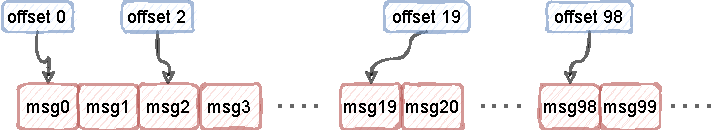
\includegraphics[scale=1.1]{obrazky-figures/02-preliminaries/02-kafka/05-offset-thing.pdf}
    \caption{Partition offset}
    \label{fig:offset}
    \end{figure}
\end{enumerate}

\subsection{Kafka Streams}

It is a stream processing tool created by the Kafka community that does expose the low level of the Consumer API and Producer API. These client APIs are very flexible, and the user can create the data processing logic he wants.
However, there is a tradeoff, and it is writing many lines of code.
Unfortunately, we cannot classify these APIs as stream processing APIs because they do not contain primitives that would classify them there, such as \emph{Local} and \emph{Fault-tolerant} state and a set of transformers that work with data (a transformer is an operator that transforms data).

In 2016, Kafka introduced the \emph{Kafka Streams API}, which solved these problems.
Inexperienced users in Kafka Streams would think it is just a matter of sending messages to and from Kafka.
Instead, we can see that Kafka has a part of Producer and Consumer, where it offers a wide range of libraries for data transformation.
Kafka streams also support two crucial operating characteristics:
\begin{enumerate}[itemsep=1mm, parsep=0pt]
    \item \textbf{Scalability} \---\ In Kafka Streams, the smallest unit of work is a single partition.
    If we want to scale the Kafka Streams application, we have to divide Topic into several partitions.
    Practically speaking, you use the Kafka Streams API to deploy multiple instances of an application, each of which will handle a subset of the work.
    For illustration, one Topic has sixteen partitions, and it is up to us how we scale it.
    One scenario could be to deploy two instances, and each of them would trade eight partitions.
    Figure \ref{fig:kafkaStreams} shows example with three partitions.
    
    \begin{figure}[!h]
    \centering
    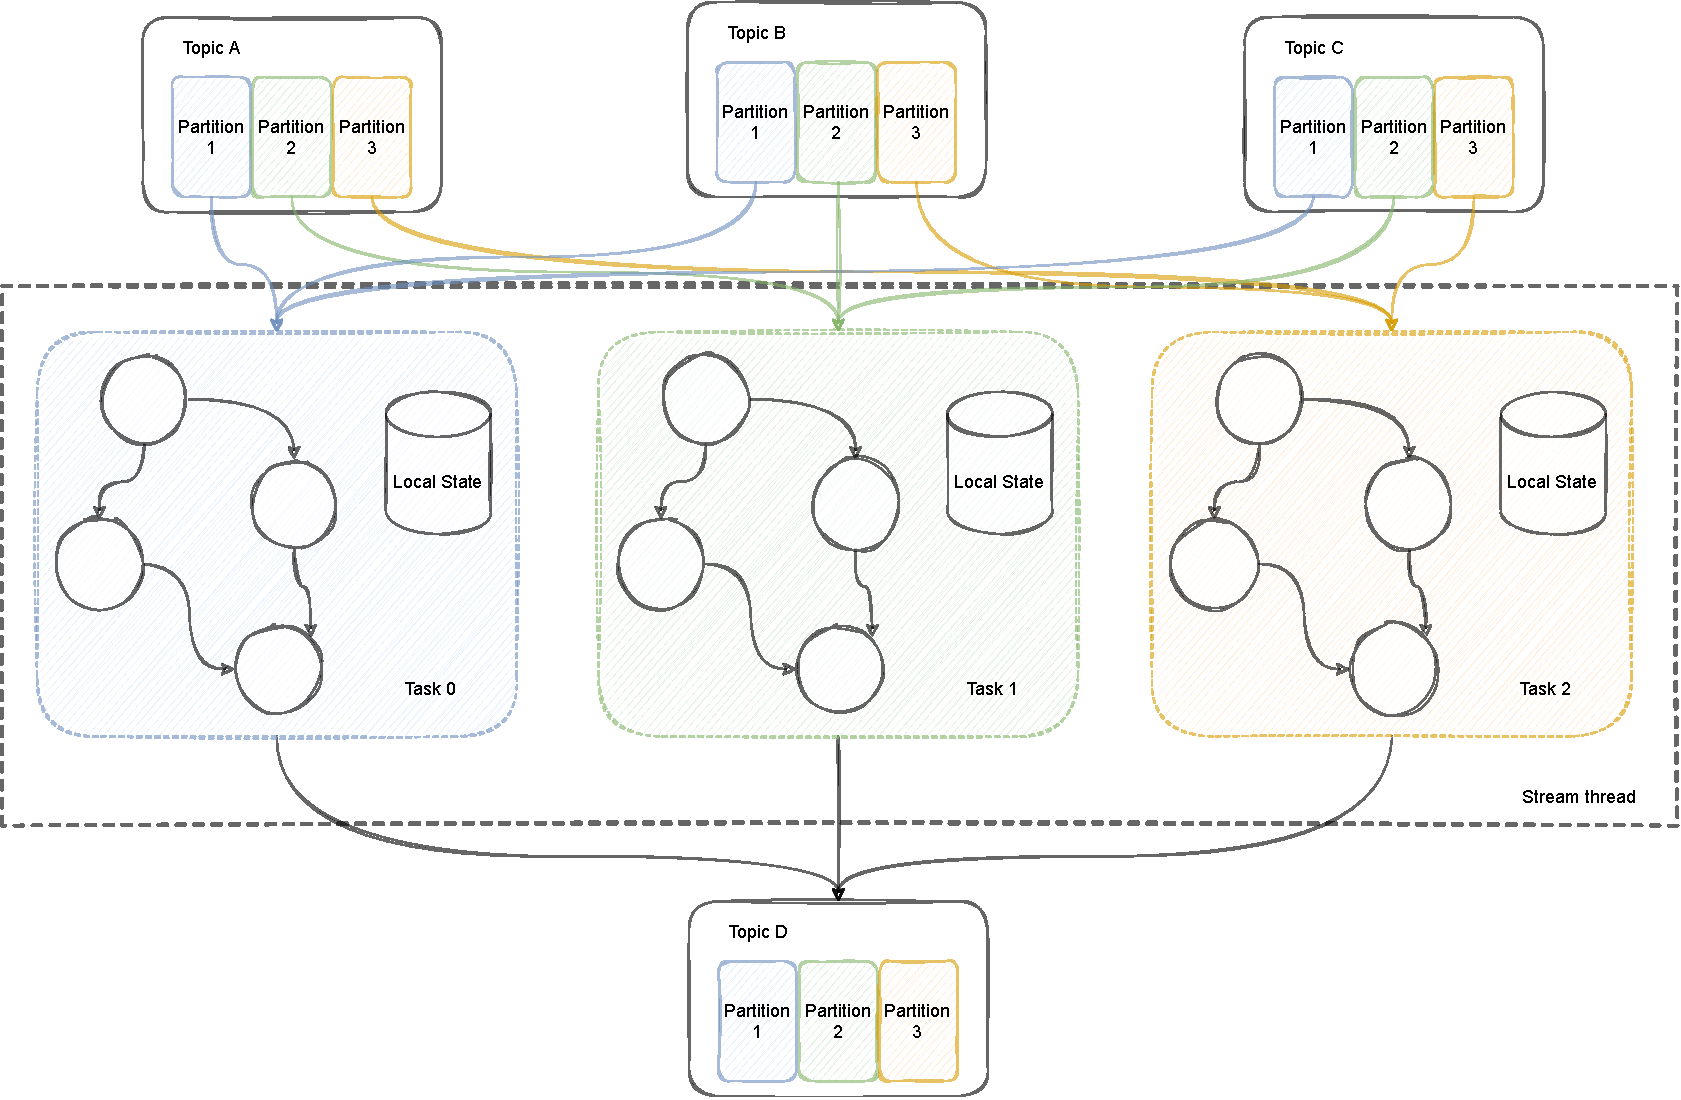
\includegraphics[scale=0.48]{obrazky-figures/02-preliminaries/02-kafka/07-kafka-streams-with-localstate,thread.pdf}
    \caption{Kafka Streams with local state stores inspired by Kafka Documentation \cite{kafkaDocumentation}}
    \label{fig:kafkaStreams}
    \end{figure}
    
    
    \item \textbf{Reliability} \---\ If an error occurs on any node, Kafka automatically distributes the load to other nodes.
    However, we must realize that if the node that crashed is the last, we may lose the data if we do not use some Volume or other external storage.
    At the same time, when the node returns the given error is corrected, Kafka will rebalance again.
\end{enumerate}

\begin{figure}[!ht]
    \centering
    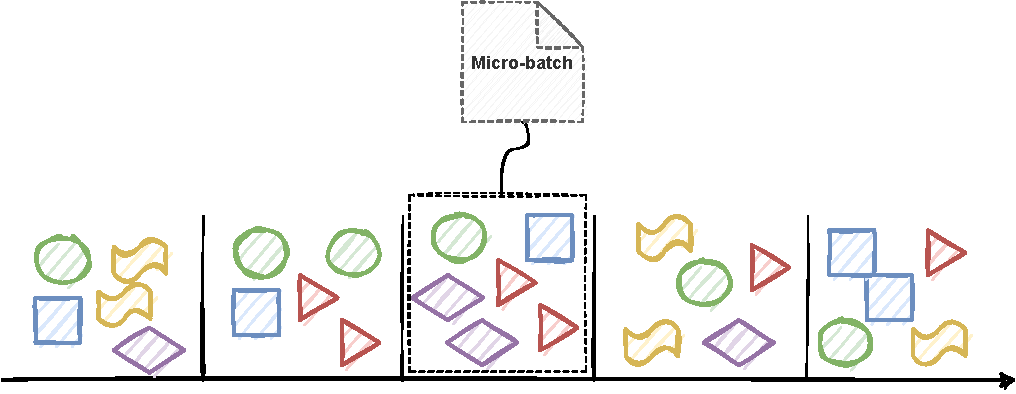
\includegraphics[scale=0.78]{obrazky-figures/02-preliminaries/02-kafka/10-kafkaStreamsProces.pdf}
    \caption{Micro-batching processing (typical for different systems) inspired by \cite{kafkaStreamsBook}}
    \label{fig:02-kafkaStreamsProcessingBatch}
\end{figure}

One of the main differences between other similar systems is the processing model that Kafka Streams offers.
These systems, such as \emph{Apache Spark Streaming}\footnote{\textbf{Apache Spark Streaming} \---\ is a extension of Spark API with many transformation methods.} or \emph{Trident}\footnote{\textbf{Trident} \---\ high-level abstraction for stream processing based on the Apache Storm. It provides multiple transformation methods such as filters, grouping, and aggregations.}, use micro-batching, which occurs very much in machine learning where work is divided into several batches.
These groups are then loaded into memory then emitted at a pre-selected interval (typically $1s$ or less).
Figure \ref{fig:02-kafkaStreamsProcessingBatch} shows a micro-batching strategy, where one can see that events are coupled into groups.
By contrast, Kafka Streams offers us event-at-a-time processing, where events are processed as soon as they arrive.
This approach gives us low latency and is considered true data streaming. Figure \ref{fig:02-kafkaStreamsProcessingEvent} illustrates the event-at-a-time processing strategy.
\begin{figure}[!ht]
    \centering
    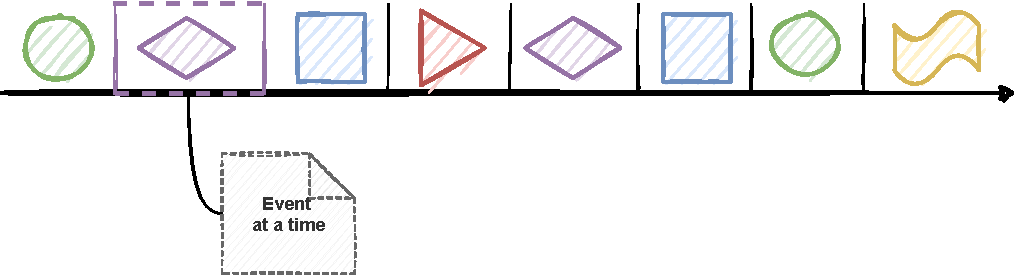
\includegraphics[scale=0.88]{obrazky-figures/02-preliminaries/02-kafka/11-kafkaStreamsProces2.pdf}
    \caption{Kafka Streams uses event-at-a-time processing inspired by \emph{Mastering Kafka Streams and ksqlDB Building real-time data systems} \cite{kafkaStreamsBook}}
    \label{fig:02-kafkaStreamsProcessingEvent}
\end{figure}

Kafka Streams is thus a set of libraries that offer developers incredible power over data processing.
Additionally, it has a model of parallelism, where the smallest logical unit is partition.
Easily scalable by either increasing or decreasing partitions, and lastly, Fault tolerance is rooted in Kafka itself (dependent on Topic replicas).
This collection of characteristics make it the perfect choice for today's data intensive applications.
These types of applications could be, for instance:
\begin{itemize}[itemsep=1mm, parsep=0pt]
    \item email tracking, monitoring,
    \item chat infrastructure (Slack), virtual assistants, chatbots,
    \item machine-learning pipelines (Twitter),
    \item smart home (IoT sensors).
\end{itemize}
There are many such types of applications.
However, what brings together all the examples is real-time data processing.

\subsection{Kafka Connect}

One of the most critical questions that every data engineer has is: "\emph{How to move data from Kafka to a datastore or vice versa?}".
Moreover how to create data pipelines that connect several systems, for instance, by selecting data from Twitter and then sending it to Elasticsearch or other external storage.
Of course, Kafka will play a middleware role in this data transfer.
We can answer the previous question and solve the data integration problem thanks to the \emph{Kafka Connect} component.

Kafka Connect offers a large number of features that are transparent to the users.
These include configuration, parallelization, error handling, and much more.
Moreover, for data integration, Kafka Connect offers two types of connectors.
Connectors are already predefined templates.
These connectors need metadata information to work.
We give this connector information such as the names of one or more Topics to follow.
In addition, these are attributes such as the connector class, number of tasks executed in parallel, and the connector URL.
The first such type of connector is Kafka Connect Source, which obtains the data from the datastore.
Information about what datastore and other metadata are provided in the connector configuration files.
In case the data in the datastore are changed, the data is automatically sent to one or more Topics.
The second type is the Kafka Connect Sink, which is analogous to the Source connector.
In the connector configuration, we define which datastore it should add data to and from which Topic it should monitor changes.
When Topic changes his state, this data is automatically pushed into the given datastore.
The simplest examples of connectors already mentioned above are the \emph{FileSource} and \emph{FileSink} connectors.

However, to properly understand Kafka Connect, it is necessary to know how the following fundamental mechanisms work:

\begin{figure}[!ht]
    \centering
    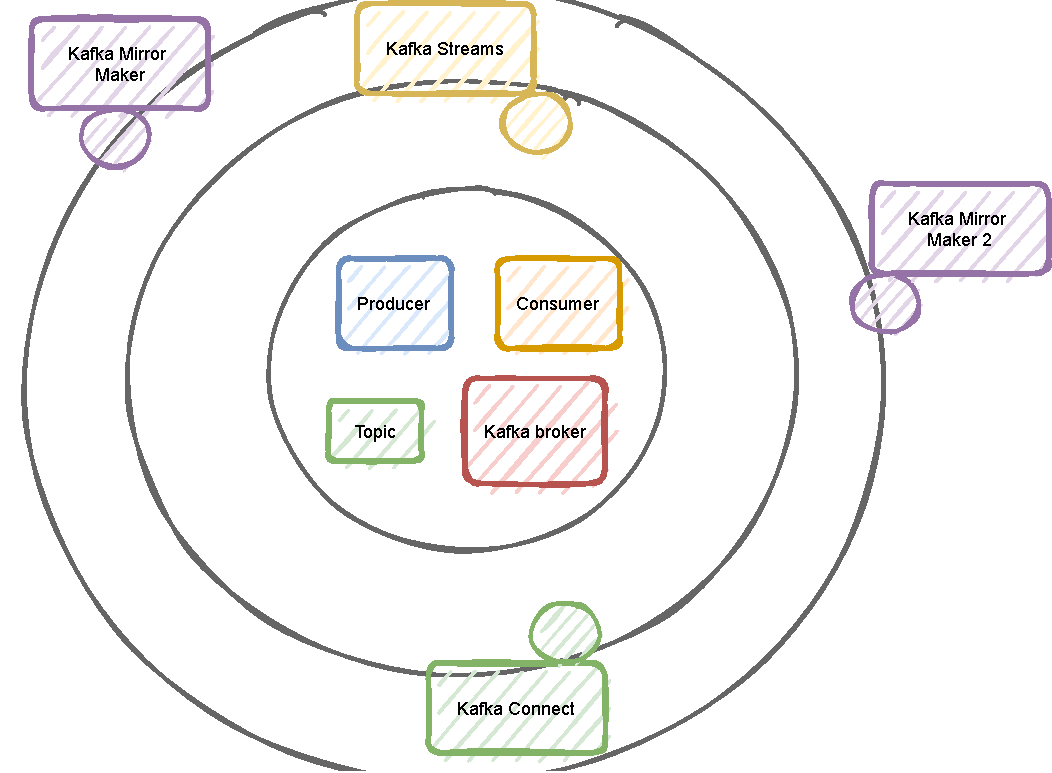
\includegraphics[scale=0.8]{obrazky-figures/02-preliminaries/02-kafka/12-all-in-one.pdf}
    \caption{The entire Apache Kafka ecosystem.}
    \label{fig:02-ecosystem-of-kafka}
\end{figure}

\begin{enumerate}
    \item \textbf{Connector} \---\ As mentioned above, the connectors are used to transfer data to and from Kafka.
    Among the essential responsibilities of connecting connectors to a given datastore, it maps the data structure that the external storage has at its disposal and decides how many tasks (threads) will run simultaneously during the transformation.
    \item \textbf{Worker} \---\ This entity is responsible for the REST API available to Kafka Connect.
    They check REST API requests and respond accordingly.
    If a worker error occurs in any way, the other workers in Kafka Connect will know this information as soon as possible and then perform rebalance and redistribute the work.
    \item \textbf{Data model and converters} \---\ Kafka Connect API contains endpoints of data objects and the scheme.
    These objects can be database tables, JSON, XML, AVRO schemas.
    Converters transform this schema to a Connect Schema object.
    Subsequently, this Connect Schema object is sent to the target system.
    There are currently many such converters available.
\end{enumerate}

All the mentioned Kafka components can be divided into three stages.
The first milestone was the emergence of a new messaging system with basic functionality and no enterprise libraries.
These included components such as Kafka Broker, Topic, Consumer, and Producer.
The lack of libraries and writing vast amounts of code in data processing brought Kafka Streams.
Kafka Connect solved data integration problems between other systems.
Finally, the Kafka Mirror Maker 2 concept came along, which improved the Kafka Mirror Maker predecessor with many capabilities.
It was a way to move data from one Kafka cluster to another.
The whole Kafka ecosystem is not trivial.
Figure \ref{fig:02-ecosystem-of-kafka} shows these stages starting with the Kafka Broker, Producer, Consumer, and Topic.
There are many other parts, such as Kafka Quotas or Kafka Rebalance features.
Nonetheless, in the thesis, we do not deal with Rebalance, Mirror Maker, or Kafka Quotas, and therefore it is not necessary to explain them in detail.
However, in case of interest, I recommend the previously mentioned literature.